\chapter{Revealing the GeV Supernova Remnant Population: The First \FermiLat{} Supernova Remnant Catalog}
\label{chap:snrCat}


%\section{Introduction}\label{snrCat:Intro}
\section{\label{snrCat:latGam}Supernova Remnants at \gam~Energies}

By the end of the its science run, \egret{} had detected 271 sources above 100\mev{}, within a minimum detection significance of 4$\sigma$, 170 of which had no clear multiwavelength counterpart, with 81 of those unidentified lying within \blat of the Galactic plane \citep{Hartman99}. The main hindrances to source identification were the numerous potential source counterparts (the \egret{} \psf{} was energy dependent, with a 68\% containment radius of ${\rm \sim 6 ^\circ}$ at 100\mev{} and smaller for higher energies) and the large \egret{} error boxes. In addition to this, the primary method for identifying a \gam{} source as an \snr{} is through a compatible angular extent with  observations at some other wavelength, thus the ability to resolve emission from an \snr{} is vital to understanding the mechanisms therein giving rise to \gam{}s. Figure \ref{fig:3EGSky} shows an \egret{} all-sky map at ${\rm E > 100 \mev}$ where the preponderance of unidentified sources and locations thereof are made clear.


\begin{figure}[h!]%[t] 
	\centering
	\makebox[\linewidth]{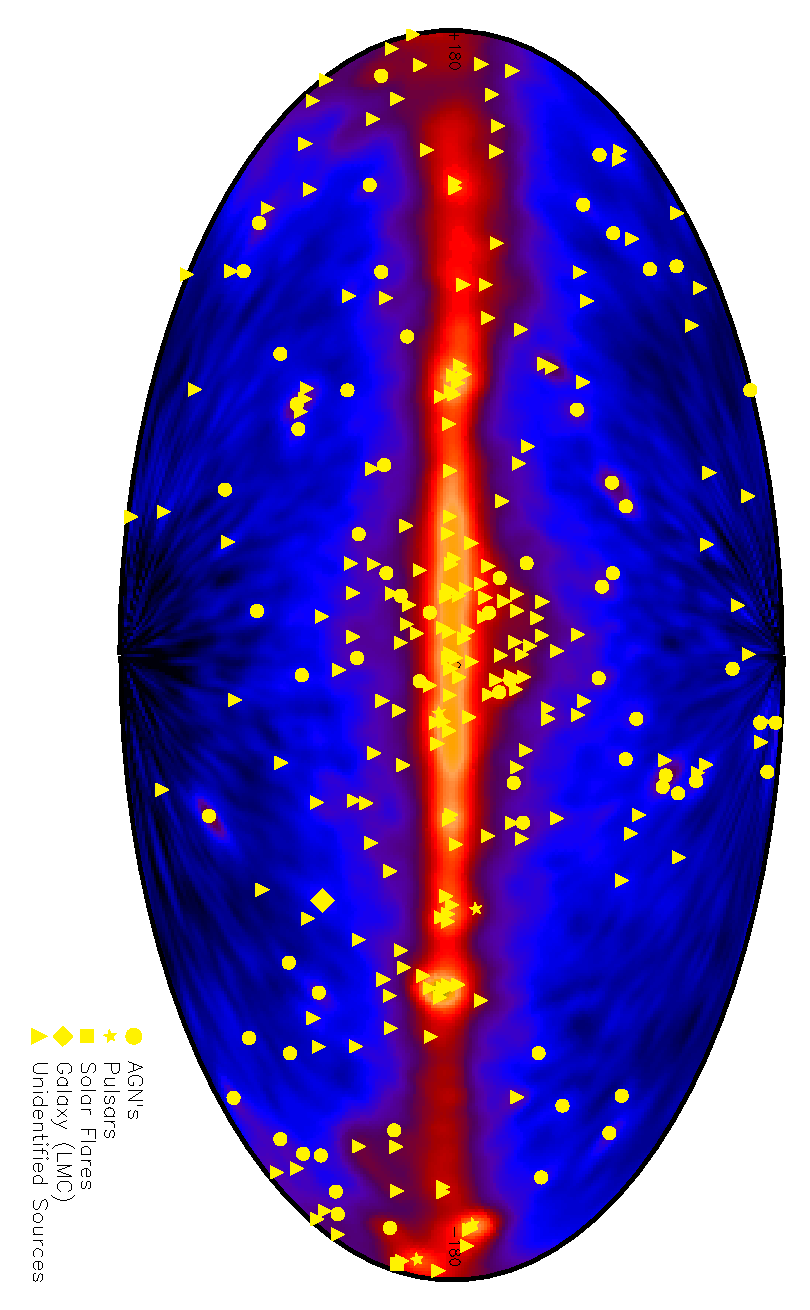
\includegraphics[width=0.8\columnwidth,angle=90]{Figures/3rd_egret_cat.eps} }
	\caption[Third EGRET catalog all-sky map.]{Third EGRET catalog all-sky map. Unidentified sources represented by triangles. Image courtesy of \url{https://heasarc.gsfc.nasa.gov/docs/cgro/images/epo/gallery/skymaps/}}
	\label{fig:3EGSky} 
\end{figure}

In spite of the difficulties in \egret{} source association, many studies have attempted correlating the unidentified \egret{} sources with various Galactic populations. In particular, several authors found strong evidence for statistical correlation between \glspl{snr} and some of the low-latitude unidentified sources \citep{Sturner95, Esposito96, Romero99}. In a review of the state of potential \snr{} /  \egret{} associations, \cite{Torres03} showed that there were 19 unidentified \egret{} sources that had an \snr~fall within its 95\% error box. Performing Monte Carlo simulations of the population of  \egret~sources, they determined that the chance probability for the 19 sources to be coincident with an \snr~was $1.05 \times 10^{-5}$, implying a probability of 0.99998 that at least one of the associations is real. Despite the statistical correlation of \egret~sources with \glspl{snr}, there were no definitive associations of an \snr~with any \egret~sources.

As the successor to \egret{}, the \lat{} was designed to improve upon its predecessor in a multitude of areas relevant to detecting \snrs{} \citep{atwood09,lat_perf}. The \lat{} has a much improved angular resolution (68\% single-photon containment radius $\sim 0.4^{\circ}$ at 1\gev{} for photons with the best quality direction reconstruction, PSF3 event type, compared to $\sim 1.7^{\circ}$ for \egret{} at the same energy), necessary to resolve \snrs{} as extended objects. The \lat{} also benefits from a superior sensitivity due to a combination of the improved \psf, larger peak effective area ($ {\rm > 9000~cm^2}$ vs. ${\rm \sim 1500~cm^2}$), wider \fov{} (2.4 sr, which is nearly 5 times that of \egret{}), and deeper, more-uniform sky exposure (afforded by the \lat's scanning observations as opposed to \egret's pointing operation). 

This bump in sensitivity results in the \lat{} detecting considerably more sources than \egret. Remarkably, within its first three months of commission, the \lat{} detected 205 sources above {\rm 10$\sigma$ significance \citep{lat_3m}, and by 11 months, 1451 sources above 4$\sigma$ \citep{1FGL}, compared to  the aforementioned 271 over the entire \egret{} mission. In fact, over its lifetime, \egret{} detected a total of about ${\rm 1.5~x~10^6}$ cosmic photons, while as of March 2016, the \lat{} has detected ${\rm \sim 863~x~10^6}$ \jamie{change this number in June} source class photons. The \lat's point-source sensitivity peaks between 1 and 10\gev{}, depending on location on the sky. \jamie{plot comparing lat to egret sensitivity?}. With its increased sensitivity and higher energy range (up to $\sim$ 2\tev{} with the recent Pass 8 event reconstruction improvements, which is nearly an order of magnitude higher than \egret{}), the \lat{} is uniquely situated to study the \gam{} morphology and spectra of \snrs{}.

Both energetic lepton interactions (\ie \ic{} radiation of relativistic electrons interacting with ambient photon fields, and nonthermal \brems{}) and hadronic processes ($\pi_0$ decay \gam{}s from \cray{} protons encountering surrounding nuclei) produce spectra observable at \gam{} energies (see Chapter \ref{chap:gamAstr} for details). While the \ic{} generating electron population is also observable through emission of radio \sync{} photons, the proton-proton interaction solely emits \gam{}s. Despite being the prime energy range to observe the effects of cosmic particle acceleration, complexities at the lower \lat{} energy range stymie \snr{} morphology studies.

The \lat{} detects a strong, soft band of diffuse emission in the Galactic plane due to the interactions of  \crs{} with interstellar material. This bright diffuse radiation combined with the multiple potential emission scenarios, broadening \psf{} at decreasing energy, and a high source density in the plane can make it difficult to spatially disentangle sources observed by the \lat{}. To circumvent these 
difficulties, the majority of the analyses undertaken in this thesis are focused on the ${\rm E \geq 1\gev}$ energy range. This energy band is ideal for probing the properties of the accelerated particle populations present in the \snr{} environment. Studies of  \snrs{}  above 1\gev{} benefit from finer \lat{} \psf{}, striking a balance between minimizing the diffuse contribution, maximizing photon sensitivity, and retaining good photon statistics. Furthermore, evolved \snrs{}  exhibit a spectral break between 1-10\gev{} \citep{Hewitt15}. Explanations for the break range from Alfv\' en wave evanescence generated by collisions of partially ionized material in \mcs{} overtaken by \snr{}  shocks \citep{Malkov11}, reflected shocks in clouds \cite{Inoue10c}, and energy-dependent diffusion from shocks \cite{Ohira11}. Studying \snrs{} in this energy range hones our capability to tackle several goals set out by the \Fermi{} team when the mission was conceived.

Two of the primary science goals of the \lat{}  are to 1. resolve the \gam~sky, uncovering the nature of the unidentified sources detected by \egret{}, and 2. to understand the mechanisms of cosmic particle acceleration \citep{atwood09}. In this chapter, we describe our efforts towards addressing these questions by studying the \gam{} emission coincident with sources comprising the population of known radio emitting \snrs{}.

Prior to this work, several individual studies with the \lat{} had successfully resolved spatially extended emission from \snrs{} \citep[and references therein]{3FGL}, yet no systematic analysis leveraging the \lat{}'s full-sky coverage had thus been attempted. We performed for the first time a uniform study of the \snrs{} in aggregate to measure the properties common to these objects. An understanding of these common characteristics allows us to assess \snrs{} as a class of \gam{} and \cray{} emitting objects and serves as the impetus for this uniform analysis of the known Galactic \snrs{}. We  report here on the published results from the \snrcat{} \citep{snrCat}.
 
 \jamie{2FGL only had 7 ID'd SNR, 4 snr, 58 spp. 3FGL had 12 SNR, 11 snr, 49 spp. I'm not sure what made some snr vs. spp. They must have all been point sources right? No known radio pwn, psr?}

%%%%%%%%%%%%%%%%%%%%%%
%%%%%%%%%%%%%%%%%%%%%%

\section{\label{snrCat:ptlk}The \ptlike{} Maximum-Likelihood Package and \srcs{}}

As described in Chapter \ref{chap:FGST}, maximum-likelihood analysis is the ideal method for determining the properties of \lat{}-observed sources due to the ``counting-experiment" nature of \FermiLat{}. The standard maximum-likelihood tools for analyzing \lat{} data are implemented via the \Fermi{} Science Tools, and in particular \gtlike{}.  Despite being the optimum method, likelihood analysis of \lat{} data is complex due to the highly non-linear performance of the instrument and can be computationally expensive. It is necessary to manage the data and response of the telescope as well as the source and background models. Furthermore, due to the broadening of the \psf{} at low energies, even when studying a single source, it is necessary to include in the model descriptions of multiple surrounding sources. The \ptlike{} binned maximum likelihood package was created to ameliorate some of these issues. Described in detail in \cite{Kerr10}, \ptlike{} is an alternate likelihood analysis framework (a collection of Python modules with additional wrappers for accessing C++ code), designed to be interactive and rapidly evaluate likelihoods.  

There are several ways in which \ptlike{} improves in efficiency compared to the Science Tools. It saves computational time, while sacrificing some accuracy,
with several assumptions and approximations, such as the \psf{} not varying strongly with photon incidence angle (allowing a single \psf{} for each individual bin), and sources having a steady flux in individual short time bins. Most importantly though, \ptlike{} varies the size of spatially binned \heal{} pixels \citep{Gorski05} according to energy. The \psf{} at lower energies is large and each energy bin can contain multiple counts, while at higher energies, the \psf{} shrinks and many pixels will not contain even a single count. \ptlike{} creates \heal{} bins that are approximately the size of the \psf{} at a given energy, and disregards empty bins to speed up the likelihood calculation.

In addition to these computational, time saving efficiencies, tools to analyze spatially extended sources have also been built into the \ptlike{} framework. Studying the position and extension of an extended source, while possible with the standard \Fermi{} Science Tools, is a cumbersome process. \gtlike{} is not capable of simultaneously maximizing the likelihood of a source's spectral and spatial parameters, so to assess the morphology of a source, an iterative process of fitting a spatially fixed source's spectrum and then varying the sources centroid and extension is required. To address the issues that arise when studying individual extended sources, \cite{Lande12} developed and validated spatial likelihood fitting tools for \ptlike{}, taking advantage of the time-saving properties built therein.

To fit the position and extension of a source, \ptlike{} assumes that the spatial and spectral distribution of a source's expected photon distribution are separable. The extended source's shape is convolved with the \lat{} \psf{} (which is a function of energy) to determine the expected distribution. Then, the {\tt minuit} numerical minimization library\citep{James75} is used to maximize the likelihood of the model by simultaneously varying the spectrum, extension, and position of the source. Various geometric surface brightness models are built into \ptlike{}, including, but not limited to a uniform intensity disk and ring, and a 2D Gaussian, with radially and non-radially symmetric versions of each. Akin to the speed optimizations mentioned previously, for radially symmetric sources, \ptlike{} calculates the angular integral of a source's expected photon distributions analytically to save computational time.

The significance of extension of a source is determined by using the \lrt{}. The \lrt{} is a statistical method to assess the goodness-of-fit of two different models. The likelihood (as described in Chapter $\S$\ref{FGST:analysis}\jamie{do this, reference cash,mattox, fisher for first use of word likelihood?}) is calculated  for two models, one of which can be reduced to the other hypothesis under certain conditions. If the more complex model can be reduced to the simpler model (called the null hypothesis), we say the simpler hypothesis is nested within the more complex. In the \lrt{}, the \ts{} is defined as: 

\begin{equation}
\rm \ts{} \equiv 2\log(\like{}(H_1)~/ \like{}(H_0)),
\end{equation}

with ${\rm H_1}$ being the more complex hypothesis and ${\rm H_0}$ the null. Applying this to the hypothesis of a spatially extended source, we can calculate the significance of a source being extended compared to that of the source being modeled as point source as:

\begin{equation}\label{eq:tsext}
\rm \ts{}_{ext} \equiv 2\log(\like_{\rm es}~/ \like_{\rm ps}) = \ts{}_{es} - \ts{}_{ps},
\end{equation}

\cite{mattox96} detail how by Wilk's theorem, the \ts{} for detection of a point source (with the null hypothesis being that with no source present, or 0 flux) should be distributed as a chi-squared  distribution in the null hypothesis for an increasing sample size, which for photon counting experiments, is the number of events relevant to the parameter being estimated. Specifically, 

\begin{equation}\label{eq:tsPdf}
\rm PDF(\ts{}) = 1/2~\chi^2_1,
\end{equation} 

where PDF(TS) is the probability distribution function for obtaining a specific value of \ts{} and $\chi^2_1$ is the chi-squared  distribution for one degrees of freedom. The factor of 1/2 arises from the fact that the flux of a source is not permitted to be zero, and since negative and positive fluctuations in a parameter's value contribute equally to the \ts{}, half of the distribution is lost with the positive flux restriction. The significance of detection is oft quoted as ${\rm \sigma \approx \sqrt{TS}}$, which is strictly valid only for $\chi^2_1$. More generally, when comparing the likelihood of two models with n degrees of freedom between them, equation \ref{eq:tsPdf} applies, but using  $\chi^2_n$ for n degrees of freedom versus one.

\cite{Lande12}, extended (and verified) this definition of \ts{} to calculating the significance of extension, replacing the source flux with its radius. The uncertainty of the extension parameter is estimated by fixing a source's position while varying the extension until the log likelihood decreases by 1/2 from the maximum value (\ie{}  1$\sigma$ errors). \jamie{use that TS vs extension figure I didn't include in the G150 paper to demonstrate where the TS drops by half from the peak?} A similar procedure is used to estimate the errors on a source's position, but rather,  fixing the extension and spectrum \citep{2FGL}. While \ptlike{} is an tool for the analyses described above, \gtlike{} is still the go-to for estimating the best-fit spectral parameters since it is expected to be slightly more accurate than \ptlike{} since it makes approximations. For the studies in this thesis, we used \ptlike{} to calculate extension and source positions, and then use the \ptlike{} results as a starting point for the likelihood parameter estimation of spectra with \gtlike{}.

With its efficient likelihood calculations, and ability to simultaneously fit both the spectral and spatial parameters of a source, \ptlike{} is ideally suited for large-scale studies (like the all-sky analyses performed for the \lat{} point source catalogs), and analyses requiring several iterations. Studying the \gam{} emission from the population of Galactic \snrs{} is precisely the sort of analysis that \ptlike{} was designed to perform. To attain the best understanding of a source of interest, the best characterization of the corresponding \roi{} is necessary. In particular, to understand the \gev{} emission from a potentially extended \snr{}, it is important to quantify the surrounding emission because of the steep energy-dependence of the \lat{} \psf{}. This can be especially challenging in dense source and strong diffuse-dominated regions, like the Galactic plane where the \snrs{} we are studying lie. We have developed an automated method for systematically locating and modeling all potential point and/or extended sources in an \roi{} using \ptlike{}. 

A typical \lat{} analysis starts by including all sources from the most recent \lat{} point source catalog and modifying the \roi{} to suit ones needs. Unmodeled emission car arise if using a dataset longer than that used in the most recent catalog or by focusing on a different energy range compared to that of the catalogs. We created a Python subclass of the primary \ptlike{} analysis object (which works within that framework, inheriting all of the class' features, while adding new functionality) to systematically and uniformly characterize sources in an \roi{} by finding residual, unmodeled emission in the region and iteratively add sources to the \roi{} to account for this emission. The main module in the designed codebase was dubbed \srcs{}. 

The general work flow of \srcs{} is to start with a model of the \roi{}, including some combination of the diffuse background components, point  and extended sources. \srcs{} reads in a residual \ts{} map or creates one on the fly if none is passed in. Residual emission is detected by finding the peak emission in the \ts{} map and adding a source to the existing \roi{} at the position of the peak pixel. Either all point or extended sources can be iteratively detected and added to the \roi{}. For the \snrcat{}, we exclusively ran \srcs{} in point source mode. Chapter \ref{sec:3FGL_ES} provides an application of \srcs{} for extended sources. 

In point source mode, a point source with a \pl{} spectrum is added to the model of the region, a likelihood fit of the \roi{} is performed, and subsequently, the source's position is localized. Similarly, in extended mode a \pl{} extended source (of any morphological form included in \ptlike{}) is added to the \roi{} with a small seed radius, and the spatial parameters of the newly added source are fit simultaneously with the spectra of the other sources already in the model. If the source has ${\rm TS_{ext} < 16}$ (equivalent to a  4$\sigma$ extension significance and validated through simulations in \cite{Lande12} as a reasonable extension detection significance), the exteded source is replaced with a point source and the iteration continues as in point source mode. To extend the functionality of \srcs{} and make it generally applicable to a multitude of \lat{} analyses, several optional methods were built in. 

One such option is to test the newly added source for signs of spectral curvature (described further in Chapter \ref{snrCat:AddSrcs}). If the source is found to show significant spectral curvature, the appropriate curved spectral model is retained, otherwise, we revert to the best-fit \pl{} model. Another option provided is to fix the new sources spectrum if it is within a given angular separation of the center of the RoI to limit the number of free parameters for the likelihood fit and aid in proper convergence. If the source of interest being studied is not central in the \roi{} it might be beneficial to free the spectral parameters of sources within a given distance of the newly added source rather than from the center of the \roi{}. This choice was also built into \srcs{}. Further, we included an option to refit the extension of any extended source already in the model at each iteration if they are within a given distance of the new (point or extended) source. Due to the broad size of the \psf{}, nearby source spectra can be influenced by each other, (particularly for extended sources) so the iterative procedure allows the likelihood to relax to a preferred value when adding new sources.

Throughout the \srcs{} process, various checks are performed to ensure that parameter values are reasonable,
the likelihood fit converges, and the procedure is generally running as expected. The range of permissible fit values for a parameter can be limited, the values of the parameters themselves can be fixed, or a consistently poorly-fit source can be automatically removed from the model. During the source localization step, if the fit goes awry and the source wanders too far from its initial position, the position of the source can be rolled back to its staring location and fixed. Checks were also included to keep track of the Galactic diffuse and isotropic emission models to ensure they were adequately fit.

The penultimate step of the iteration is to produce various diagnostic plots and output information about the fits, the spectral and spatial parameters of each source in the model, and other relevant information such as the \ts{} of the source and loglikelihood of the fit. Finally, a new residual \ts{} map of the region is created and the source addition procedure repeats until a given threshold in \ts{} is reached. The peak pixel \ts{} found in the residual \ts{} map does not necessarily decrease monotonically, as is expected of the actual \ts{} of successive sources as more of the emission is accounted for and the model improved. \jamie{figue showing this?} Since the peak pixel TS can fluctuate a bit, to ensure that we do not miss significant sources in the \roi{}, we continue adding sources until the \ts{} threshold is reached for some number of successive sources (discussed further in \ref{snrcat:AddSrcs}). After sources are no longer being added to the region, we iteratively remove souces with \ts{} less than a given threshold (typically ${\rm TS < 16}$, again see Chapter \ref{snrcat:AddSrcs}) starting with the lowest \ts{} sources first. As each source is removed, we refit the \roi{}, including any extended sources close to the removed source. When the TS of all sources in the \roi{} are above threshold, we deem the emission in the \roi{} to be sufficiently characterized.

In the following sections, we detail the application of \srcs{} to studying the \gev{} Galactic \snr{} population and describe the analysis and results presented in \cite{snrCat}.

%The peak pixel \ts{} value determined from the \ts{} map and used as the seed position for a newly added source is not the same as the \ts{} of the source itself. The peak pixel does not necessarily decrease monotonically, as is expected of the \ts{} of successive sources as more of the emission is accounted for and the model improved We can see how they differ by recalling that a \ts{} map is created by placing a point source at each grid location in the map and finding the \ts{} of the source at that specific pixel. While the \ts{} of the source itself (log likelihood ratio of the hypothesis with the source and without) is determined 

\jamie{show some example region map with unmodeled sources and then the final result where sources were filled in? Extended vs not extended (just use 2FHL vs this chapter for that. Many sources vs sparse). Something like, Figure blah is a residual TS map showing an example of what a typical \roi{} might look like before running \srcs{} and after} 
\jamie{talk about the prelim SNR cat tests with 6 SNRs here? See what was said about the tests in the SNR cat}

%%%%%%%%%%%%%%%
%%%%%%%%%%%%%%%

\section{Galactic Supernova Remnants}\label{sncat:SNRSelection}
\jamie{from SNRcat}
In this work we focus on the 279 currently known Galactic SNRs. They are derived from the $274$~SNRs noted in the catalog of \citet[hereafter Green's catalog]{Green09}, plus five additional SNRs identified following its publication. 
All but $16$ of these SNRs have been identified by their radio synchrotron emission, so their centroids and extensions are primarily determined from the radio. When the radio detection is not securely identified through the synchrotron emission, positional information is obtained from the optical, X-ray, or TeV observations that identified the SNR, as noted in Green's catalog. The catalog is thought to be complete down to a $1$\,GHz radio surface brightness limit of $\approx 10^{-20}$\,W\,m$^{-2}$\,Hz$^{-1}$\,sr$^{-1}$ (i.e.\,$1$\,MJy\,sr$^{-1}$). However, selection effects are known to bias radio surveys against the identification of radio faint and small angular size remnants \citep{Green04,Brogan06}. We note that as this work neared completion, a revised catalog of $294$~SNRs was published \citep{Green14}, representing only a small increase ($<10\%$) over the previous catalog.


%%%%%%%%%%%%
%%%%%%%%%%%%

\section{Analysis Methods}\label{snrcat:AnalysisMethod}
\jamie{from SNRcat}
To systematically analyze the \FermiLat{} \gam{} data, we apply a maximum likelihood \citep{mattox96} framework to \rois{} centered on known SNRs \citep{Green09}. For each SNR, we begin by constructing a model for the spectral and spatial dependence of the \gam{} emission which includes significant point sources in the RoI. We then test for the existence of a \gam{} source near the center. This includes determining the most likely position and extension of the candidate source and testing for spectral curvature, rather than assuming it follows a \pl{} across the energy range studied. In cases where we find no significant source associated with the SNR, we calculate upper limits on the flux. We calculate both statistical and systematic errors, where the latter are estimated from both the uncertainty in the effective area and the effects of changing the \iem{}, which accounts for \gam{}s produced by CR interactions with interstellar gas and radiation fields in the Milky Way. 

This analysis uses both the standard Science Tools (version 09-32-05), including \gtlike{}, and the \ptlike{} analysis package~\citep{Kerr10} which has been developed and verified for characterizing source extension for \FermiLat{} data \citep{Lande12}. $\S$\ref{snrcat:Data} describes our data selection; $\S$\ref{snrcat:AddSrcs} details our new method for automatically finding point sources in the \FermiLat{} \g-ray emission; and $\S$\ref{snrcat:DetectMethod} discusses the detection method.

\section{Data Selection}\label{snrcat:Data}
\jamie{from SNRcat}
This catalog was constructed using 3 years of LAT survey data from the Pass~$7$~(P7) ``Source'' class and the associated P7V6 \irf{}.This interval spans $36$\,months, from $2008$\,August\,$4$ to $2011$\,August\,$4$ (mission elapsed time $239557417-334108806$). The Source event class is optimized for the analysis of persistent LAT sources, and balances effective area against suppression of background from residual misclassified charged particles. We selected only events within a maximum zenith angle of $100$\degr{} and use the recommended filter string ``DATA\_QUAL==1 \&\& LAT\_CONFIG==1'' in {\tt gtmktime}\footnote{See LAT data selection recommendations at: \url{http://fermi.gsfc.nasa.gov/ssc/data/analysis/documentation/Cicerone/Cicerone_Data_Exploration/Data_preparation.html}.}. 
The P7 data and associated products are comparable to  those used in the other \gam{} catalogs employed in this work. We used the first three years of science data for which the associated IEM is suitable for measuring sources with extensions $>2$\degr \footnote{See the LAT caveats, \url{http://fermi.gsfc.nasa.gov/ssc/data/analysis/LAT_caveats.html}, particularly those for the IEM developed for Pass~$7$ reprocessed data described in \url{http://fermi.gsfc.nasa.gov/ssc/data/access/lat/Model_details/FSSC_model_diffus_reprocessed_v12.pdf}.}. A detailed discussion of the instrument and event classes can be found in \cite{atwood09} and at the \Fermi{} Science Support Center\footnotemark[1].

For each of the 279 SNRs we modeled emission within a $10$\degr{}\,radius of the SNR's center. As a compromise between number of photons collected, spatial resolution, and the impact of the \iem{}, we chose $1$\,GeV as our minimum energy threshold. The limited statistics in source class above $100$\,GeV motivated using this as our upper energy limit. 

To avoid times during which transient sources near SNRs were flaring, we removed periods with significant weekly variability detected by the \Fermi{} All-sky Variability Analysis (FAVA) \citep{fava13}. We conservatively defined a radius within which a flaring source may significantly affect the flux of a source at the center. We take this distance to be the radio radius of an SNR plus $2.8$\degr, corresponding to the overall $95\%$~containment radius for the \FermiLat{} point spread function (PSF) for a $1$\,GeV photon at normal incidence \citep{lat_perf}. The time ranges of FAVA flares within this distance were removed in $23$~RoIs, leaving $\geq 98.9\%$ of the total data in each RoI.

%%%%%%%%%%%%%%%%%%
%%%%%%%%%%%%%%%%%%
\section{Input Source Model Construction}\label{snrcat:AddSrcs}
\jamie{from SNRcat}
To characterize each candidate SNR we constructed a model of \gam{} emission in the RoI which includes all significant sources of emission as well as the residual background from CRs misclassified as \gam{}s. We implemented an analysis method, built upon the \srcs{} method described in \ref{snrCat:ptlk}, to create and optimize the 279 models for each of the $279$~RoIs. For each RoI, we initially included all sources within the $10$\degr{} RoI listed in the \twofgl{} \citep{2FGL}, based on $2$\,years of Source class data. To this we added pulsars from the \twopc{} \citep{2PC}, based on $3$\,years of source class data, with 2PC taking precedence for sources that exist in both. 
For the diffuse emission we combined the standard \iem{} corresponding to our P7 data set, gal\_2yearp7v6\_v0.fits, with the standard model for isotropic emission, which accounts for extragalactic diffuse \gam{} emission and residual charged particles misclassified as \gam{}s. Both the corresponding isotropic model, iso\_p7v6source.txt, and the IEM are the same as used for the 2FGL catalog analysis\footnote{Further details on the diffuse emission models are available at \url{http://fermi.gsfc.nasa.gov/ssc/data/access/lat/BackgroundModels.html} \jamie{and in Chapter blah]}}. 

Compared to 2FGL, we used an additional year of data and limited the energy range to $1-100$\,GeV. This can result in different detection significances and localizations than previously reported in 2FGL. To account for these effects, we recreated the RoIs' inner $3$\degr{}\,radius regions, which encompass the radio extents of all known SNRs, observed to be $\leq 2.6$\degr{} and allows a margin for the LAT PSF. The weighted average $68\%$~containment radius of the LAT PSF for events at $1$\,GeV is $\sim0.7$\degr{} \citep{lat_perfo}. We note that this implicitly assumes that an SNR's GeV extent should not be more than about an order of magnitude larger than its radio extension and also note that the selection biases stated in Green's catalog limit the range of known SNRs' radio extensions. 

To build the inner $3$\degr{}\,radius model of each RoI, we first removed all sources except identified \agn{} and pulsars, whose positions on the sky are independently confirmed by precise timing measurements \citep{2PC}. Retained AGN were assigned their 2FGL positions and spectral model forms. Pulsars' positions and spectral forms were taken from 2PC. 2FGL sources identified or associated with SNRs are removed when they lie within the inner $3$\degr{}. 

Using \srcs{}, we generated a \ts{} map via \ptlike{} on a square grid with $0.1$\degr{}\,$\times$\,$0.1$\degr{} spacing that covers the entire RoI. At the position of the maximum TS value, we added a new point source with a Power Law (PL) spectral model:
\begin{equation}
\label{eqn:PL}
\frac{dN}{dE} = N\frac{(-\Gamma+1)E^{-\Gamma}} {E_{\rm max}^{-\Gamma+1} - E_{\rm min}^{-\Gamma+1}}
\end{equation}
where $N$ is the integrated photon flux, $\Gamma$ is the photon index, and $E_{\rm min}$ and $E_{\rm max}$ are the lower and upper limit of the energy range in the fit, set to $1$\,GeV and $100$\,GeV, respectively.
We then performed a maximum likelihood fit of the RoI to determine $N$ and $\Gamma$ and localized the newly added source. 
The significance of a point source with a PL spectral model is determined by the $\chi^2_n$ distribution for $n$ additional degrees of freedom for the additional point source, which is typically slightly less than~$\sqrt{\textrm{TS}}$

To promote consistent convergence of the likelihood fit, we limited the number of free parameters in the model. For sources remaining after the removal step, described above, we freed the normalization parameters for the sources within $5$\degr{} of the RoI center, including identified AGN and pulsars. For 2FGL sources between $5$\degr{} and $10$\degr{}, we fixed all parameters. The spectrum of the IEM was scaled with a PL whose normalization and index were free, as done in 2FGL. For the isotropic emission model, we left the normalization fixed to the global fit value since the RoIs are too small to allow fitting the isotropic and Galactic IEM components independently. The isotropic component's contribution to the total flux is small compared to the IEM's at low Galactic latitudes.

After localizing them, the new sources were tested for spectral curvature. In each of the four~energy bands between $1$ and $100$ GeV, centered at $1.8$, $5.6$, $17.8$ and $56.2$\,GeV, we calculated the TS value for a PL with spectral index fixed to $2$ and then summed the TS values. We refer to this as $\mathrm{TS_{band fits}}$. A value for $\mathrm{TS_{band fits}}$ much greater than the TS calculated with a PL ($\mathrm{TS_{PL}}$) suggests that, with a more rapid calculation, that the PL model may not accurately describe the source. Analogously to 2FGL, we allow for deviations of source spectra from a PL form by modeling sources with a log-normal model known colloquially as LogParabola or logP:
\begin{equation}
\newcommand{\pfrac}[2]{\left(\frac{#1}{#2}\right)} \frac{dN}{dE} = N_0\pfrac{E}{E_b}^{-(\alpha + \beta\log(E/E_b))}
\label{eqn:logP}
\end{equation}
where $N_0$ is the normalization in units of photons/MeV, $\alpha$ and $\beta$ define the curved spectrum, and $E_b$ is fixed to $2$\,GeV\footnote{Note: $E_b$ is a scale parameter which should be set near the lower energy range of the spectrum being fit and is usually fixed, see \citet{massaro04}}. If $\mathrm{TS_{band fits} - TS_{PL}} \geq 25$, we replaced the PL spectral model with a logP model and refit the RoI, including a new localization step for the source. We retained the logP model for the source if the global log likelihood across the full band improved sufficiently: 
$\mathrm{TS_{curve}} \equiv 2 ($\logL{}$_{\mathrm{logP}}-$\logL{}$_{\mathrm{PL}}) \geq 16$. 
Otherwise we returned the source to the PL model which provided the better global log likelihood. Across all RoIs, less than $2\%$ of the newly added sources retained the logP model. 

We continued iteratively generating TS maps and adding sources within the entire RoI until additional new sources did not significantly change the global likelihood of the fit. The threshold criterion was defined as obtaining $\mathrm{TS < 16}$ for three consecutively added new sources, denoted as $\mathrm{N_{TS < 16} = 3}$. Despite iteratively adding a source at the location of the peak position in the TS map, the TS values of new sources may not decrease monotonically with iteration for several reasons. First, source positions were localized after fitting the RoI and generating the TS map. Second, some added sources were fit with a more complex spectral model than a simple PL. Finally, when creating the TS map, we fixed the source's spectral index to $2$, whereas when adding the actual source to the model, we allowed its index to vary. 

The specific value of $\mathrm{N_{TS < 16} = 3}$ was chosen to avoid missing sources with $\mathrm{TS \geq 25}$ (the threshold commonly used for source detection in LAT data), and to optimize computation time. We tested the threshold by selecting eight representative SNRs from both complex and relatively simple regions of the sky, with both hard and soft spectral indices. The eight chosen regions were:

{\bfseries SNR043.3-00.2 (W49B)}: A relatively simple region and test case that was previously detected as a point-source  \snr{} \citep{Abdo10-W49B}

{\bfseries SNR034.7-00.4 (W44)}: Previous LAT studies showed the SNR had a GeV extension slightly larger than the radio size as well as surrounding\gev{} emission from nearby extended sources associated with molecular clouds \citep{Abdo10-W44,Uchiyama12-W44Vicin}

{\bfseries SNR078.2+02.1 (gamma Cygni)}: A complex region containing the \snr{} an embedded pulsar, several nearby pulsars, and a large diffuse structure known as the Cygnus cocoon which is believed to be a bubble of hot gas acting as a source of freshly accelerated \crs{} \citep{Ackermann12-CygnusCR,Ackermann11-CygnusCocoon}. The region serves as a test of how robust \srcs{} is in one of the more extreme \rois{}. Despite the complexity of the region, \cite{Lande12} detected \gev{} emission co-spatial with the radio \snr{}.

{\bfseries SNR027.4+00.0 (Kes 73), SNR031.9+00.0 (3C391), SNR292.2-00.5, SNR332.4-00.4 (MSH 16-51), SNR205.5+00.5 (Monoceros)}: These five  sources were found to have large fitted extensions (greater than twice the radio radius of the \snr{}) in preliminary \snrcat{} pipeline runs so were included to understand this occurrence.

We applied the procedure detailed above to the test RoIs using a criterion of $\mathrm{N_{TS < 16} = 6}$ and counted how many $\mathrm{TS \geq 25}$ sources would be excluded if a smaller $\mathrm{N_{TS < 16}}$ criterion was used. Figure \ref{fig:NTSthresh} shows how reducing the threshold to $\mathrm{N_{TS < 16} = 3}$ cut only one significant source in any of the regions. A further criteria to validate the value of $\mathrm{N_{TS < 16}}$ used in this paper was that the spectrum of a source of interest (\ie{} the central extended \snr{} in and \roi{}) or extension was robust to the addition of nearby sources. In Figures \ref{fig:threshFlux}, \ref{fig:threshIndex}, and  \ref{fig:threshSigma}, we show an example of the evolution of the flux, index, and extension of \snr{} gamma Cygni  as subsequent sources are added.  Sources were added to the ROI until $\Delta(\logL{}) < 8$, 6 times in a row, and see that while a significant source added close to the \snr{} can affect the fit of the extended source, these fits stabilize before our threshold is reached. Since the maximum number of sources added in any test RoI was $38$, the minimum $14$, and the total number of sources added across all test regions was $221$, we chose to use $\mathrm{N_{TS < 16} = 3}$ for the full sample of 279 \rois{}. 

\begin{figure}[ht!]
	\centering
	\makebox[\linewidth]{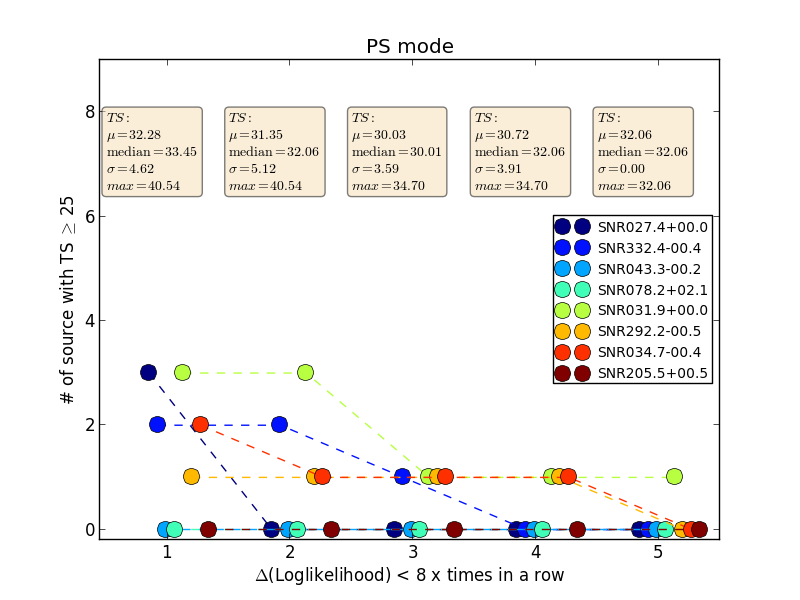
\includegraphics[width=1.0\columnwidth]{figures/aboveThreshPSgt25.png}}
	\caption[Histogram of the number of signiciant soures remaining in each of the 8 test \roi{} for iterations in which $\Delta(\logL) < 8$]{Histogram of the number TS $\geq$ 25 sources remaining in each of the 8 test \roi{} for iterations in which $\Delta(\logL) < 8$ (\ie{} TS $<$ 16). Points are offset for each SNR for clarity. The text boxes detail statistics for the values of TS of significant sources for the 8 studied SNRs for each corresponding value on the x-axis.}
	\label{fig:NTSthresh}
\end{figure}

\begin{figure}[ht!]
	\centering
	\makebox[\linewidth]{\includegraphics[width=1.0\columnwidth]{figures/{ES_1_Flux_SNR078.2p02.1_ES_noColor}.png}}
	\caption[Gamma Cygni flux evolution for successive \srcs{} iterations]{Flux evolution of the extended source coincident with \snr{} gamma Cygni (labeled ES 1 in the figure) as successive sources are added to the ROI.  Dotted line is first time $\Delta(\logL) < 8$, dashed line shows the final threshold for this test study. \jamie{these are the wrong figures, they go out 8 times}}
	\label{fig:threshFlux}
\end{figure}

\begin{figure}[ht!]
	\centering
	\makebox[\linewidth]{\includegraphics[width=1.0\columnwidth]{figures/{ES_1_Index_SNR078.2p02.1_ES_noColor}.png}}
	\caption[Gamma Cygni index evolution for successive \srcs{} iterations]{Same as Figure \ref{fig:threshFlux} but for the \pl{} spectral index.}
	\label{fig:threshIndex}
\end{figure}

\begin{figure}[ht!]
	\centering
	\makebox[\linewidth]{\includegraphics[width=1.0\columnwidth]{figures/{ES_1_Sigma_SNR078.2p02.1_ES_noColor}.png}}
	\caption[Gamma Cygni extension evolution for successive \srcs{} iterations]{Same as Figure \ref{fig:threshFlux} but for the radius of a uniform, symmetric disk.}
	\label{fig:threshSigma}
\end{figure}



To allow for proper convergence of the likelihood fit, we reduced the number of free parameters prior to each new source addition. If the previously added source was between $3$\degr{} and $5$\degr{} of the center of the RoI, just its normalization was freed, and if greater than $5$\degr{} all its source parameters were fixed.
To avoid having newly added sources overlap with pulsars, we deleted new sources from the RoI if they were within~$0.2$\degr{} of a \g-ray pulsar and refit the pulsar in the $1-100$\,GeV range following the 2PC conventions. 
2PC modeled pulsar spectra as a PL with an exponential cutoff (PLEC),
\begin{equation}
\newcommand{\pfrac}[2]{\left(\frac{#1}{#2}\right)} \frac{dN}{dE} = N_0 \pfrac{E}{E_0}^{-\Gamma} \exp\left(-\frac{E}{E_c}\right)^{b},
\label{eqn:PLEC}
\end{equation}
where \textit{$N_0$} is the normalization factor, \textit{$\Gamma$} is the photon spectral index, \textit{$E_c$} the cutoff energy, and $b$ determines to the sharpness of the cutoff. 2PC assessed the validity of fixing $b$ to $1$ in Equation~\ref{eqn:PLEC} (PLEC1) by repeating the analysis using a PL model, as well as the more general exponentially cut off PL form, allowing the parameter $b$ in Equation~\ref{eqn:PLEC} to vary. For the pulsar spectra in this analysis, we compared the maximum likelihood values for spectral models with and without a cutoff and with and without the value of $b$ being free, via $\mathrm{TS_{cut}} \equiv 2 ($\logL{}$_{\mathrm{PLEC1}}-$\logL{}$_{\mathrm{PL}})$ and $\mathrm{TS}_{b} \equiv 2 ($\logL{}$_{\mathrm{PLEC}}-$\logL{}$_{\mathrm{PLEC1}})$ to determine which to use. If $\mathrm{TS_{cut}} < 9$ is reported for the pulsar in 2PC then a PL model is used. If TS$_{\mathrm cut} \geq 9$, we then check to see if the cutoff energy fit in 2PC lies within the restricted energy range of $1-100$\,GeV used in this work. For pulsars with cutoffs $\geq 1$\,GeV, we then use the PLEC model if TS$_{\mathrm b} \geq 9$, and the PLEC model with cutoff freed otherwise. For those pulsars with cutoffs less than 1 GeV the spectral parameters are fixed to the 2PC values.

To complete the construction of our point source RoI model, we took the output of the previous steps and removed all sources with TS~$< 16$. This final model was then used as the starting model for analyzing candidate SNR emission. We conservatively allow sources with TS down to $16$ $(\sim4\,\sigma)$ in order to account for the effects of at least the brightest sub-threshold sources on the parameter fits for the other sources in the model. Furthermore, while the SNR analysis method described in the chapter \ref{snrcat:DetectMethod} is allowed to remove sources, it cannot add them. Thus we start from a set of sources designed to allow the final model to capture all significant emission within the central region. To corroborate our method of systematically adding sources to a region, we compare our RoI source models with those found by the 2FGL approach in Chapter \ref{snrcat:addSrcs2FGL}. 

%%%%%%%%%%%%%%%%%%%%%%%%
%%%%%%%%%%%%%%%%%%%%%%%%

\section{Comparison of Source Models with 2FGL}
\label{snrcat:addSrcs2FGL}

\jamie{from SNRcat}This SNR catalog was constructed using $3$~years of P7 Source class data in the energy range $1-100$\,GeV, whereas 2FGL used $2$\,years of data over the larger energy range $0.1-100$\,GeV. The differences in observing time and energy range resulted in residual, unmodeled emission in some RoIs as well as changes to some 2FGL sources' spectral model, position localization, and detection significance. Here we compare the input source models constructed for this catalog, described in Chapter \ref{snrcat:AddSrcs}, with 2FGL to better understand the \srcs{} method's ability to describe the regions studied. Since we rederive the input source model only within a $3\degr$\,radius of the center of each RoI, we consider sources only inside that radius.

Given the data set differences, in each RoI we expect similar but not identical numbers of sources relative to those in 2FGL.
Figures~\ref{fig:2FGLvAddSrcs} and \ref{fig:2FGLvAddSrcsAssoc} show the numbers of significant (TS\,$\geq 25$) 2FGL sources and derived input model sources (excluding 2FGL identified AGN and pulsars kept in the input model) in individual RoIs as 2D histograms. In Figure~\ref{fig:2FGLvAddSrcs}, the number of sources in the derived input model is typically greater than the number of 2FGL sources that are significant at $1-100$\,GeV. 73 of the 279 RoIs studied contain at least one of the the 12 extended 2FGL sources. Since 2FGL extended sources were removed from the inner $3\degr$ of each RoI, and this region was repopulated with point sources, we can detect multiple point sources inside the extent of any removed extended 2FGL sources. This decomposition of extended sources, combined with the longer data set and different energy range compared to 2FGL, contribute to the high ratio of input model to 2FGL sources in some RoI, which demonstrates the need to rederive the source model. 

\begin{figure}[h!]
	\centering
	\makebox[\linewidth]{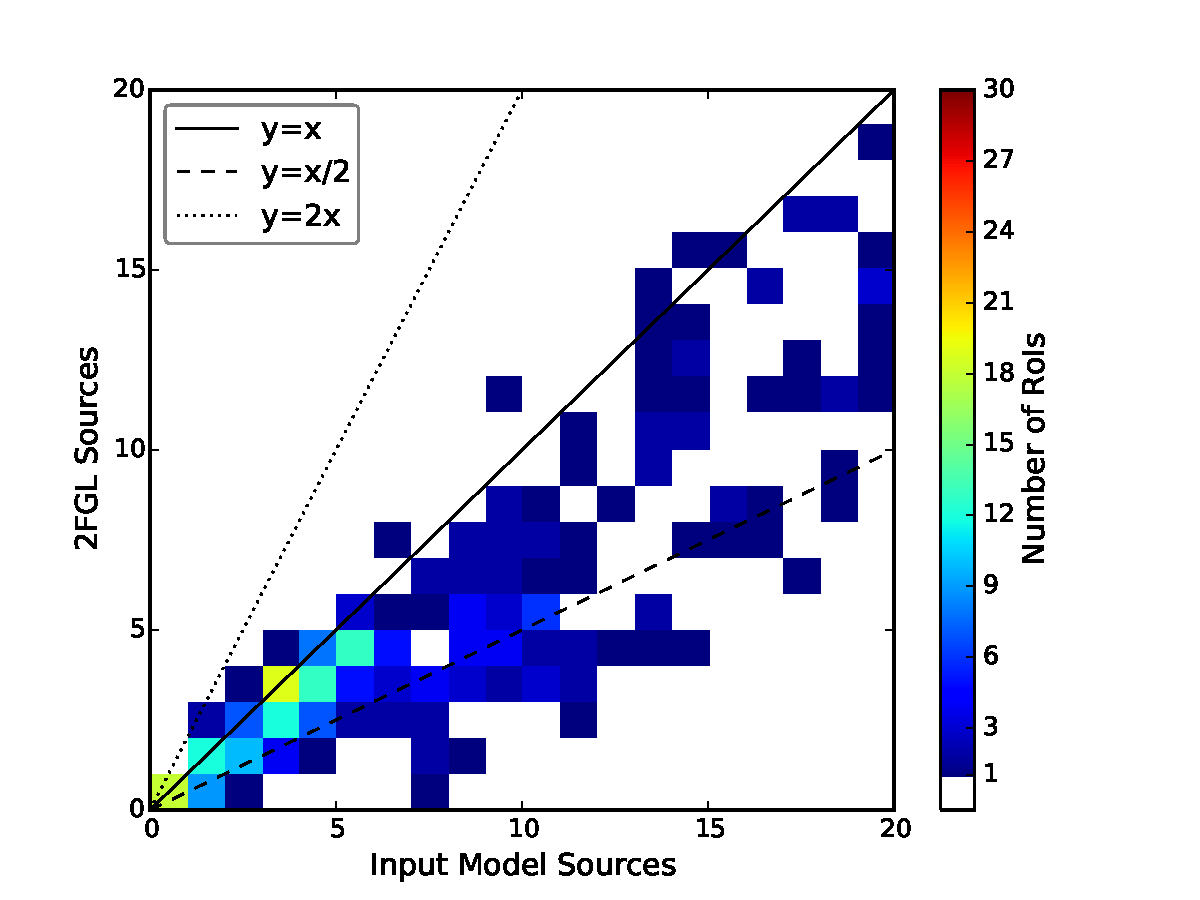
\includegraphics[width=1.0\columnwidth]{figures/addSrcs_2FGLnoAGNPSR_TSgt25_in3deg_2dhist_maj.pdf}}
	\caption[Comparison of the number of 2FGL sources with with the number of newly added input model sources.]{Comparison of the number of 2FGL sources with TS$_{1-100\,\mathrm{GeV}} \geq 25$ (excluding AGN and pulsars) with the number of newly added input model sources in the present analysis, for sources within $3$\degr{} of the center of each RoI. The color scale shows the number of RoIs with a particular combination of numbers of 2FGL sources and new sources. White corresponds to no RoI with that combination of source counts.}
	\label{fig:2FGLvAddSrcs} 
\end{figure}

To more accurately represent the 2FGL sources being reproduced in the central $3\degr$, in Figure~\ref{fig:2FGLvAddSrcsAssoc} we limited the input model sources to those within $0.2\degr$ (approximately the width of the core of the $10$\,GeV PSF) of a 2FGL source, effectively excluding input sources that are not co-spatial with a 2FGL source. Here we see that the majority of 2FGL sources have counterparts in the rederived set. As a region's complexity increases, seen as an increase in numbers of 2FGL sources, up to about half of the 2FGL sources may not have counterparts within $0.2$\degr. Given that in these same regions we have more new sources than 2FGL sources, as seen in Figure~\ref{fig:2FGLvAddSrcs}, we find as expected that the longer data set with improved statistics at higher energies, where the angular resolution of the LAT is the best, allows us to add new sources to account for newly significant excesses in these complex regions. Additionally, sources with low TS in 2FGL are particularly susceptible to having a newly added source which may start at a similar position but then localize further than $0.2\degr$ from the 2FGL source. 

Thus, we find that the method developed and used here produces a model which reproduces the 2FGL sources as expected, including differences that trend as anticipated given the longer data set and modified energy range, yielding better spatial resolution. The new method thus provides reasonable representations of the regions being modeled as input for the final analysis.

\begin{figure}[h!]
	\centering
	\makebox[\linewidth]{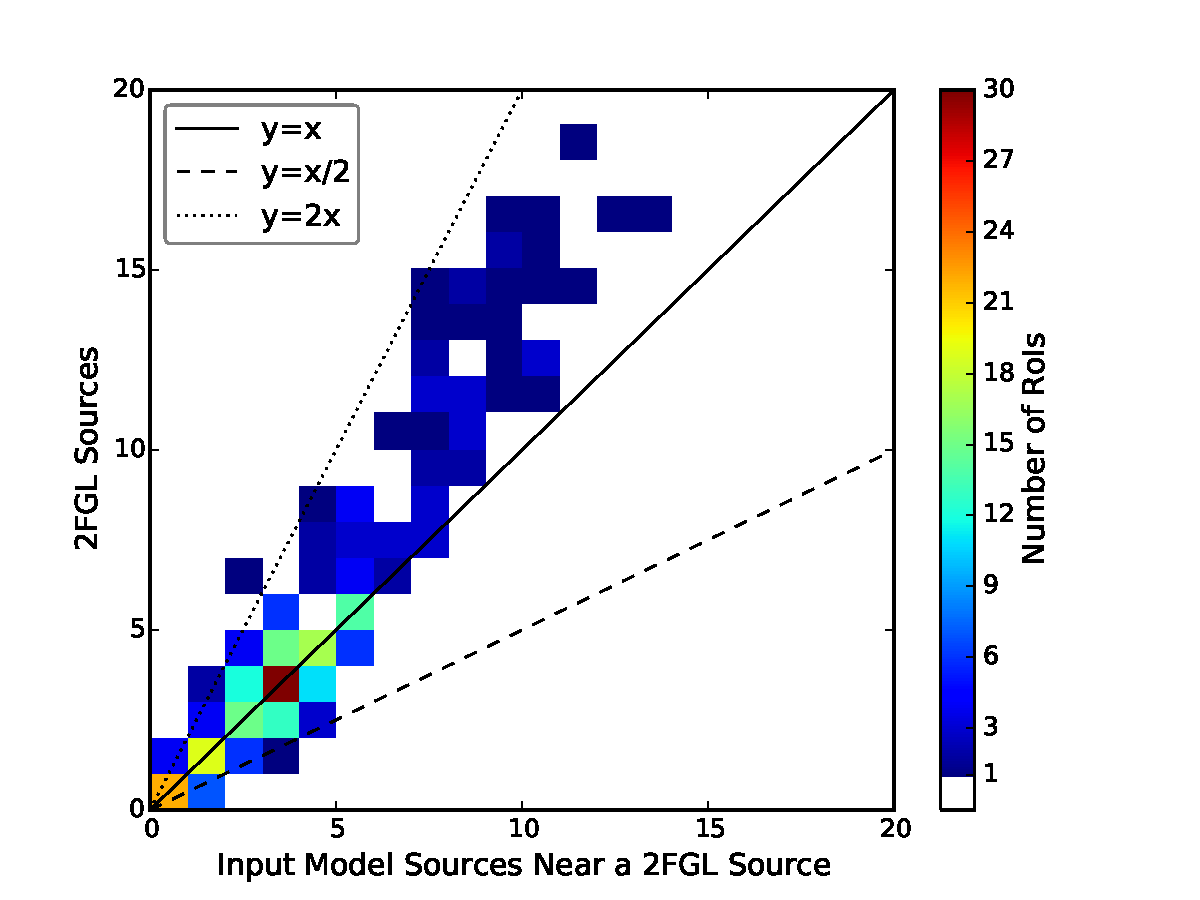
\includegraphics[width=1.0\columnwidth]{Figures/addSrcsWassoc_2FGLnoAGNPSR_TSgt25_in3deg_2dhist_maj.pdf}}
	\caption[Same as Figure~\ref{fig:2FGLvAddSrcs}, including only input model sources lying within $0.2$\degr{} of a 2FGL source.]{Same as Figure~\ref{fig:2FGLvAddSrcs}, including only input model sources lying within $0.2$\degr{} of a 2FGL source.}
	\label{fig:2FGLvAddSrcsAssoc} 
\end{figure}

%%%%%%%%%%%%%%%%%%%%
%  ANALYSIS SECTION
%%%%%%%%%%%%%%%%%%%%

\section{Detection Method}\label{snrcat:DetectMethod}

\jamie{from SNRcat}For each SNR, we characterize the morphology and spectrum of any \gam{} emission that may be coincident with the radio position reported in Green's catalog. This was achieved by testing multiple hypotheses for the spatial distribution of \gam{} emission: a point source and two different algorithms for an extended disk. The best fit was selected based on the global likelihoods of the fitted hypotheses and their numbers of degrees of freedom. The hypothesis with the best global likelihood was then evaluated using a classification algorithm described in \cite{snrCat} to determine whether the radio SNR could be associated with the detected \gam{} emission. 

Spatial coincidence is a necessary but not sufficient criterion to identify a \gam{} source with a known SNR. The detection of spatially extended \gam{} emission increases confidence in an identification, especially if GeV and radio sizes are similar, as has been observed on an individual basis for several extended SNRs \citep[e.g.][]{Lande12}. The LAT has sufficient spatial resolution to detect many Galactic SNRs as extended. Figure~\ref{fig:size_hist_p} shows the distribution of radio diameters from Green's catalog. Vertical dashed lines show the minimum detectable extension for sources with flux and index typical of those observed in this catalog, based on simulations using the P7V6 IRFs~\citep{Lande12}. The minimum detectable extension depends not only on the source's flux and spectrum, but also the flux of the background, which was estimated by scaling the average isotropic background level by factors of 10 and 100 to be comparable to the Galactic plane. As figure~\ref{fig:size_hist_p} illustrates, roughly one third of the known Galactic SNRs may be resolved by the LAT if they are sufficiently bright GeV sources.

\begin{figure}[h!]
	\centering
	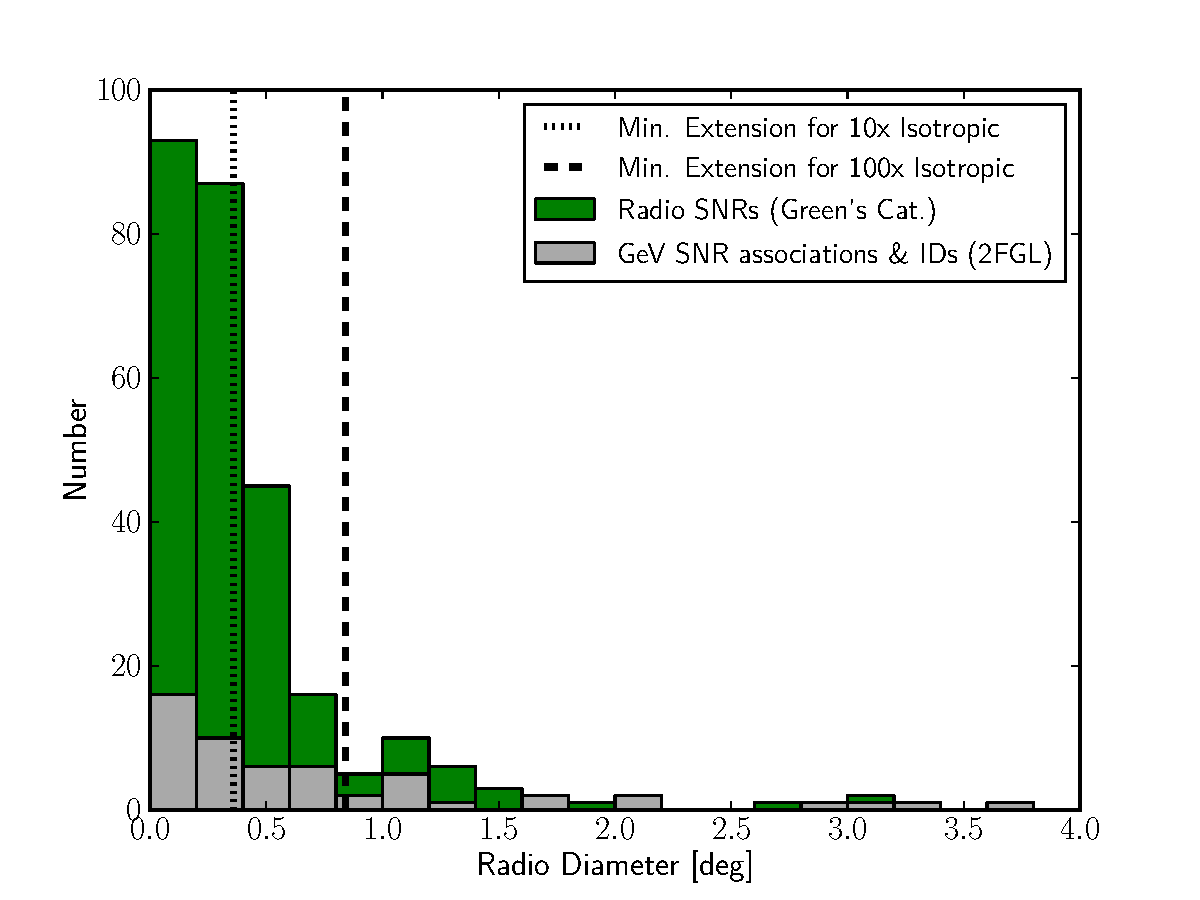
\includegraphics[width=1.0\columnwidth]{figures/size_hist_p.pdf} 
	\caption[Distribution of SNR radio diameters from Green's catalog]{Distribution of SNR radio diameters from Green's catalog. The vertical dashed lines indicate the minimum detectable extension for a source with a photon flux of $10^{-8}$\,ph\,cm$^{-2}$\,s$^{-1}$ in the $1-100$\,GeV energy range and a PL index of $-2.5$, from simulations of $2$\,years of data and the P7V6 IRFs \citep{Lande12}. In that work, simulations using $10$x and $100$x the isotropic background level (thin-dotted and thick-dashed lines) are used to estimate a reasonable background range for sources in the Galactic plane.\jamie{idk what plots are ok or not to include from papers I am an author on. I didnt make this plot, but I made the first version of it that inspired this one. Should I specifically include a comment for these plots that state they're from the snr cat vs ones not in the paper?}}
	\label{fig:size_hist_p}
\end{figure}

In order to determine the best representation for each SNR, we analyzed each SNR-centered RoI using multiple hypotheses for the spatial and spectral form. We used \ptlike{}~\citep{Kerr10} to compare PL and logP spectral forms, to compare point source versus extended source hypotheses, and to analyze the robustness of sources near the extended source.

For each hypothesis, we started with the input model described in Chapters \ref{snrcat:Data} and~\ref{snrcat:AddSrcs}. We removed sources falling within the SNR's radio disk unless they had been identified as an AGN or pulsar, as described in Chapter \ref{snrcat:AddSrcs}. We then proceeded to evaluate the following point and extended source hypotheses. For the point source hypothesis, a point source with a PL index initialized to $2.5$ was placed at the radio centroid of the SNR. The positions, spectral index, and spectral normalization of the point source were then fit. As for the initial input model described in Chapter \ref{snrcat:AddSrcs}, we tested the source for spectral curvature. To test the extended source hypothesis, we employed two separate procedures. Both employed a uniform disk model initially placed at the center of the RoI with a radius equal to that observed in the radio. In the first procedure, called the ``disk" hypothesis, we fit both the position and extension of the disk, as well as tested for spectral curvature. A second procedure, which results in a model we call the ``neardisk" hypothesis, additionally examines the significance of sources nearby the disk, removing those which are not considered independently significant and refitting the disk position and radius. This procedure is described in Chapter \ref{snrcat:LocExtSpec}.

Having evaluated these hypotheses, we compared the global likelihood values of the final extended hypothesis and of the point source hypothesis to determine which model had the largest maximum likelihood. If the source is significant in the best hypothesis, the model parameters are reported as Tables 1 and 2 in \cite{snrCat}. If no hypothesis had a significant \gam{} source coincident with the radio SNR, we calculated the upper limit on the flux from a region consistent with the radio SNR, described in Chapter \ref{snrcat:FluxULs}, and report  the results in Table 3 in \cite{snrCat}. \jamie{should I include the tables here? only if they're short, or abridged. I should def include the dist table because I did that work}

\subsection{Localization, Extension, and Spectral Curvature}\label{snrcat:LocExtSpec}

\jamie{from SNRcat}To test our hypotheses, we combined the initial model of point sources (Chapter \ref{snrcat:AddSrcs}) and the Galactic and isotropic diffuse contributions (Chapter \ref{snrcat:Data} and \ref{snrcat:AddSrcs}) with a test source at the center of each RoI. All sources that fell within the radio SNR radius other than previously identified AGN or pulsars were removed, as was done for the input source model (Chapter \ref{snrcat:AddSrcs}). We note that multiple point sources removed within a single radio SNR radius may represent substructure within the source itself. This process conservatively assigns the majority of the flux to a single source, rather than decomposing it. We optimized the position of the test source with \ptlike{}, iteratively allowing other model parameters to vary. For all hypotheses, the normalizations of all sources within $5$\degr{} of the radio SNR center were fit while all other spectral parameters were fixed. The parameters for sources outside $5$\degr{} were also fixed.

For the point source hypothesis, a point source was placed at the radio centroid of the SNR. For the disk hypothesis, a uniform disk with radius equal to the radio radius was placed at the center. In both hypotheses, the normalization, index, and position of the candidate source were fit. For the disk hypothesis, the extension was also fit. Previous analyses of a range of possible Galactic SNR sources with similar data sets \citep[e.g.][]{Lande12} typically showed no differences in global likelihood significant enough to justify choosing a Gaussian over a uniform disk template or vice versa. In addition, there was typically little difference in spectral parameters for the two spatial forms. For simplicity and clarity, we thus test only the uniform disk hypothesis. We allowed the localization to wander up to  $5$\degr{} in the fits as a reasonable upper limit on what might later be associated with the SNR. This is roughly twice the radius of largest radio SNR.

We included an additional disk hypothesis in which we recalculated the significance of each nearby point source. Because neighboring sources can influence the best fit disk parameters, we iteratively evaluated the significance of the neighboring source by calculating TS$_{\rm nearby}$, defined as twice the difference between the model's log-likelihood (\logL{}) with the nearby point source and the model without the source, as determined by \ptlike. Starting from the fitted disk model, for each neighboring point source we refit the position, extension, normalization, and spectrum of the uniform disk after removing the source. A nearby source was considered to be significant and thus kept if TS$_{\rm nearby} \geq 9$. Each point source was evaluated individually, starting with the closest point source and extending radially outward to all sources within $1$\degr{} of the furthest edge of the SNR's radio disk. The final result of this iterative process is called the ``neardisk" hypothesis which, for cases where neighboring source(s) were removed, can have different best fit disk parameters. As a final step we refit the region with \gtlike, using the neardisk model.

We chose the best extended source hypothesis by comparing the final disk and neardisk \gtlike{} \logL{} values. Since the neardisk hypothesis can have fewer degrees of freedom, we chose the final disk hypothesis only if $2\times$(\logL{}$_{\rm disk}$-\logL{}$_{\rm neardisk}$) $\geq 9$. Otherwise, we used the neardisk model as the final extended source hypothesis, hereafter referred to as the ``disk hypothesis''.

In some cases a point source could not be localized starting at the SNR center. If the \ptlike{} localization failed to converge when starting at the SNR center, we placed the candidate at the position of the most significant source removed from within the radio SNR radius and followed the procedure outlined above. For $69$~RoIs there was either no source removed within the radio SNR or localization failed. For $31$~RoIs, the candidate found had a TS~$<1$ and was removed from the model so as not to cause instabilities in the minimization. If the disk hypotheses converged and the final candidate was significant (TS~$\geq 25$) in both the localization and spectral fits, the best extended hypothesis was selected. 

Prior to the final fit of the region, sources were tested for spectral curvature using $\mathrm{TS_{band fits} - TS_{PL}}\geq~25$. If this criterion was satisfied then we replaced the PL spectral model with a logP model and refit the RoI. The final spectral model was selected, as for the input model, by comparing the \logL{} values, in this case $\mathrm{TS_{curve}} \geq 16$, as defined in Chapter \ref{snrcat:AddSrcs}. Seven sources were found to be significantly better fit by a logP spectrum. To obtain final spectral parameters, we performed a final fit using the standard likelihood analysis tool \gtlike. The normalization and index parameters were constrained to lie within a physically reasonable range. 

%%%%%%%%%%%%%%%%%%%%%%%%%%%%%%%%%%%

We determined the final RoI model by selecting the most likely hypothesis based on a comparison of the \gtlike{} global \logL{} of the point source hypothesis with the most likely extended source hypothesis. An extended hypothesis was considered significantly more likely if $\mathrm{TS_{ext}}$ was $\geq 16$, where $\mathrm{TS_{ext}}$ is defined as twice the difference between the \logL{} of the final model from the disk hypothesis and that of the point source hypothesis, $\mathrm{TS_{ext}} =  2 ($\logL{}$_{\mathrm{disk}}-$\logL{}$_{\mathrm{point}})$, as in~\citet{Lande12}. Otherwise, if the point source itself had TS\,$>25$, we chose the point source hypothesis. In cases in which the optimization for the position of the point source did not converge but an extended disk was detected, we calculated the global \logL{} of the region without any source and with a point source at the center of the extended source. We then use the latter value to calculate $\mathrm{TS_{ext}}$ reported in Table 1 in \cite{snrCat}. For these candidates, if the source was significantly extended in both cases, we select the extended hypothesis. If none of the criteria were met, the candidate was considered undetected and we calculated an upper limit on the flux. Both the upper limits and flux calculation are described in the following subsection.

\subsection{Fluxes and Upper Limits}\label{snrcat:FluxULs}

\jamie{from SNRcat}Fluxes in the $1-100$\,GeV band are determined using the standard analysis tool \gtlike{} by a final fit of the model chosen to have the overall maximum likelihood characterization of the morphology and spectrum of the candidate source from the analysis detailed in Chapter \ref{snrcat:DetectMethod} and \ref{snrcat:LocExtSpec}. For those RoIs where no significant source was detected, we computed Bayesian upper limits on the flux using the method in described in \citet{Helene83} excluding any overlapping sources in the model that have not been identified as AGN or pulsars, as described in Chapter \ref{snrcat:AddSrcs}. As a spatial model we used a uniform disk equal in position and radius to that reported in Green's catalog. We assumed the spectral model to be a PL and report upper limits for indices of $2.0$ and $2.5$ at $95\%$ and $99\%$ confidence levels. The choice of indices was motivated by the distribution of PL indices for classified sources. The results are reported in \cite{snrCat}.

%%%%%%%%%%%%%%%%%%%%%%%%
%%%%%%%%%%%%%%%%%%%%%%%%


\section{Summary}\label{snrCat:summ}
In this chapter, we have presented results from the publication of the \snrcat. Application of addSrcs adding point sources to characterize emission in an\roi. Give more details on validation and testing than was given in the paper, as well as details on the code. Work on fitting single extended source, present some work on detected SNRs and population properties, implications for total power in cosmic rays (don't focus on this because it wasn't where I contribute the most). Mock catalog contributions. Testing with extended sources or don't mention too much because we decide not to apply it here?

With its unprecedented sensitivity and angular resolution above 1\gev, the \lat~provides for the first time the opportunity to distinguish SNR-emitted photons from their backgrounds, and  to unambiguously detect and identify dozens of \glspl{snr}. \jamie{maybe this is for the intro/abstract because it's a little vague}

The \lat{} is uniquely situated to address these goals and definitively detect and identify dozens \snrs

Focus our efforts on

\section{Scratch}
has the spatial and spectral sensitivity to resolve

good spatial and spectral 


talk about how much "power" comes from the higher energy  range,

EGRET point source sensitivity is ${\rm \sim1x10^{-7}}\flux{}$
\url{http://fermi.gsfc.nasa.gov/science/instruments/table1-1.html} get this number from somewhere else


\jamie{somewhere I should also say that identifying an extended source as such gives better spectra, see 2FHL}

\cite{Thomson93}, egret observed a total of 1.5 million celestial \gam{}

\jamie{ Fermi goals: 1. Resolve the \gam~sky: the origins of diffuse emission and the nature of unidentified sources: Source identification through good source localization, measurement of spectra across broad energy range, nearly continuous monitoring of the sky for temporal variability
	2. Understand the mechanisms of particle acceleration in celestial sources:}

\jamie{understanding accel plus identification of the potential SNRs motivates the SNR cat }

\jamie{snrs as source of Galactic cosmic rays, and thus as drivers of Galactic evolution}

-what's to gain from studyng the population vs individual?

-constraint on CR energy density in the Galaxy

-do the observed g-ray properties match those
of models?

-like index etc?

\jamie{Another assumption to speed things up is that the PSF doesn't vary too much with event incidence angle in individual bins. To ensure this even more, events with a reconstructed angle > 66.4deg (cos theta = 0.4) are removed (idk why this angle)}

This section is about the tools (and intricacies there in) developed to study SNRs with Fermi

The addSrcs framework extends/exploits pointlike 

addSrcs in this section or merged into the next one?

I need to stress that this is not just a tool developed, but there's an art and finesse to it (talk about the problems we overcame), there was much iteration.

tool plus knowledge to get the best result

what are the aspects of addSrcs tht needed knowhow, finagling

, \ts{} map creation and extension fitting.
\jamie{assume I've mentioned \ts{} maps already}  For these reasons, we utilized \ptlike{} to perform an analysis of 

we endeavored to take 

First something about the SNR cat, and wanting to uniformly study the regions around SNRs, maybe this is a new section
to facilitate the characterization of the sky

what are some motivations for various addSrcs decisions 

How to distinguish addSrcs from how addSrcs was applied to the SNR cat. For the SNRcat, it was addSrcs in PS mode with specifics relevant to the SNR cat needs (like what?)

tested pipeline with 6 sources (I have the tests somewhere, see old Fermi symp poster, Gal Evo too)

The min bias line is specifically for the SNR cat since we removed catalog sources....intended to minimize possible bias introduced by the initial model for an ROI (e.g 2FGL) It is  used to derive the input sources model for the SNR catalog. The goal of this work is to use this "add sources" method to aid in characterization of GeV emission near SNRs and nearby molecular clouds.

left to do in this section:

figure out which other sections to pull from.

I think I might just take the first part of the results of the catalog, and summarize the comparison results (so maybe just the most relevant population plots and points about correlation?)

The one other part that I need to write is about the 8 sources tested on. pull from pres, and poster and confluence. 

Reread the chapter, figure out what other plots to include


First par of 3.1 about how we classify. Summarize some of the relevant catalog results of section 3.2. There's no real reason to include the catalog tables I think. Parts of 3.2.1 3.2.2, 3.2.3 just to highlight which sources were newly detected. 

What to include from section 4? I didn't make these plots, but I contributed to the pipeline script and gave advice on things. 

For the mock snrCatalog, I didn't do the analysis, but I ran addSrcs on the mock sources. maybe there's not much to say about this though.

Section 5? It's not my work, but I participated in discussions, edited text in the section a little bit. I think something needs to be included from this because one of the points of the paper was to see what we could say about the total energy in CR in the Galaxy

Parts of conclusion
